% Made up for the tikra benchmark.
\usetikzlibrary{shapes.misc}
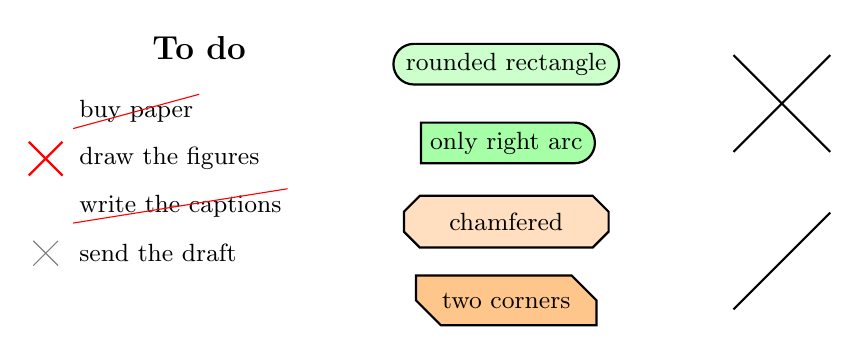
\begin{tikzpicture}[font=\small, item/.style={anchor=west, inner sep=2pt}]
  \node[font=\bfseries\large] at (1.6,0.8) {To do};
  \node[item, strike out, draw=red] at (0,0) {buy paper};
  \node[item] at (0,-0.6) {draw the figures};
  \node[item, strike out, draw=red] at (0,-1.2) {write the captions};
  \node[item] at (0,-1.8) {send the draft};
  \node[cross out, draw=red, thick, minimum size=4mm] at (-0.35,-0.6) {};
  \node[cross out, draw=gray, minimum size=3mm] at (-0.35,-1.8) {};
  % the shapes of shapes.misc
  \node[rounded rectangle, draw, thick, fill=green!20, minimum width=2.6cm] at (5.5,0.6) {rounded rectangle};
  \node[rounded rectangle, rounded rectangle left arc=none, draw, thick, fill=green!35] at (5.5,-0.4) {only right arc};
  \node[chamfered rectangle, draw, thick, fill=orange!25, minimum width=2.6cm] at (5.5,-1.4) {chamfered};
  \node[chamfered rectangle, chamfered rectangle corners={north east, south west}, chamfered rectangle xsep=4mm,
        draw, thick, fill=orange!45] at (5.5,-2.4) {two corners};
  \node[circle, draw, thick, fill=cyan!15, cross out, minimum size=1.2cm] at (9,0.1) {};
  \node[circle, draw, thick, fill=cyan!15, strike out, minimum size=1.2cm] at (9,-1.9) {};
\end{tikzpicture}
